\documentclass{book}

\usepackage[utf8]{inputenc}
\usepackage[T1]{fontenc}
\usepackage[french]{babel}
\usepackage[dvipsnames]{xcolor}
\usepackage[top=1.5cm, bottom=2.5cm, left=3cm, right=2cm]{geometry}
\usepackage{lmodern}
\usepackage{ae, aecompl}
\usepackage{fancyhdr}

\usepackage{amssymb}
\usepackage{amsmath}
\usepackage{mathrsfs}
\usepackage{amsthm}
\usepackage{url}
\usepackage{listings}
\usepackage{stmaryrd}
\usepackage{array}
\usepackage{multirow}
\usepackage{verbatim}
\usepackage{bookmark}

\usepackage{soul}
\usepackage{ulem}
\usepackage{graphicx}
\usepackage{eso-pic}
\usepackage{float}

\usepackage{makeidx}
\usepackage{glossaries}

\newcommand{\rouge}{\textcolor{red}}
\newcommand{\bleu}{\textcolor{blue}}
\newcommand{\p}{\vspace{0.2cm}}

\addto\captionsfrench{\renewcommand{\chaptername}{Partie}}
\floatplacement{figure}{!ht}
\floatplacement{table}{!ht}

\newtheorem{definition}{Définition}[chapter]

\lstset{
	language=Python,        				% choix du langage
	basicstyle=\footnotesize,       % taille de la police du code
	numbers=left,                   % placer le numéro de chaque ligne à gauche (left)
	numberstyle=\normalsize,        % taille de la police des numéros
	numbersep=7pt,                  % distance entre le code et sa numérotation
	breaklines=true
}

\lstdefinelanguage{INI}
{
  basicstyle=\ttfamily\small,
  columns=fullflexible,
  tag=[s]{[]},
  tagstyle=\color{Dandelion}\bfseries,
  usekeywordsintag=true,
  morecomment=[l]{;},
  commentstyle=\color{gray}\ttfamily,
  alsoletter={=},
  ndkeywords={=},
	numbersep=7pt,
  ndkeywordstyle=\color{green}\bfseries
}[html]

\makeindex
\makeglossaries

\makeatletter
\def\@ecole{école}
\newcommand{\ecole}[1]{
  \def\@ecole{#1}
}

\def\@specialite{Spécialité}
\newcommand{\specialite}[1]{
  \def\@specialite{#1}
}

\def\@ED{\'{E}cole Doctorale}
\newcommand{\ED}[1]{
  \def\@ED{#1}
}

\def\@doctorat{Doctorat}
\newcommand{\doctorat}[1]{
  \def\@doctorat{#1}
}

\def\@adresse{Adresse}
\newcommand{\adresse}[1]{
  \def\@adresse{#1}
}

\def\@directeur{directeur}
\newcommand{\directeur}[1]{
  \def\@directeur{#1}
}

\def\@encadrant{encadrant}
\newcommand{\encadrant}[1]{
  \def\@encadrant{#1}
}
\def\@jurya{}{}{}
\newcommand{\jurya}[3]{
  \def\@jurya{\textbf{#1},	& #2	& #3\\}
}
\def\@juryb{}{}{}
\newcommand{\juryb}[3]{
  \def\@juryb{\textbf{#1},	& #2	& #3\\}
}
\def\@juryc{}{}{}
\newcommand{\juryc}[3]{
  \def\@juryc{\textbf{#1},	& #2	& #3\\}
}
\def\@juryd{}{}{}
\newcommand{\juryd}[3]{
  \def\@juryd{\textbf{#1},	& #2	& #3\\}
}
\def\@jurye{}{}{}
\newcommand{\jurye}[3]{
  \def\@jurye{\textbf{#1},	& #2	& #3\\}
}
\def\@juryf{}{}{}
\newcommand{\juryf}[3]{
  \def\@juryf{\textbf{#1},	& #2	& #3\\}
}
\def\@juryg{}{}{}
\newcommand{\juryg}[3]{
  \def\@juryg{\textbf{#1},	& #2	& #3\\}
}
\def\@juryh{}{}{}
\newcommand{\juryh}[3]{
  \def\@juryh{\textbf{#1},	& #2	& #3\\}
}
\def\@juryi{}{}{}
\newcommand{\juryi}[3]{
  \def\@juryi{\textbf{#1},	& #2	& #3\\}
}
\makeatother

\makeatletter
\newcommand{\pagedegarde}{
  \newgeometry{top=2.5cm, bottom=1cm, left=2cm, right=1cm}
  \begin{titlepage}
    \begin{center}
      
\includegraphics[width=0.2\textwidth]{annex/logo_UCA.eps}
      \hfill
      
\includegraphics[width=0.4\textwidth]{annex/isima.eps}\\
      \vspace{1cm}
      % \vspace{1cm}
      \vspace{1cm}
        {\huge RAPPORT DE STAGE}\\
      \vspace{0.3cm}
        {\small Norvège\\}
      \vspace{1cm}
        {\large 2\up{ème} année F4}\\
      \vspace{0.5cm}
      	\textit{Projet réalisé par}\\
      \vspace{0.5cm}
        {\Large {\bfseries \@author}} \\
      \vspace{0.5cm}
      	le \@date \\
      \vfill
         {\huge \color[rgb]{0,0,1} \bfseries{\@title}} \\
      \vfill
          Tuteur de Stage : {\bfseries \@directeur}\\
          Co-encadrant de Stage : {\bfseries \@encadrant}\\
      \vfill
    	\begin{tabular}{l l l}
    		\large{\textbf{Jury}}\\
    		\@jurya
    		\@juryb
    		\@juryc
    		\@juryd
    	% 	\@jurye
    	% 	\@juryf
    	% 	\@juryg
    	% 	\@juryh
    	% 	\@juryi
    	\end{tabular}
    	\vfill

      \begin{flushright}
        durée : 120 heures
      \end{flushright}

    	\@adresse
    \end{center}
  \end{titlepage}
  \restoregeometry
}


\title{\'Etat de l'art}
\author{Julien \textsc{Feuillas}}
\directeur{Arvid \textsc{Lundervold}}
\encadrant{Alexander \textsc{Lundervold}}
\adresse{\bsc{Isima} 1 rue de la Chebarde, Aubière 63170}
\jurya{Arvid \bsc{Lundervold}}{Professeur UiB}{Maître de Stage}
\juryb{Murielle \bsc{Mouzat}}{Professeure ISIMA}{Communication}
\juryc{Vinvent \bsc{Barra}}{Professeur ISIMA}{Tuteur ISIMA}
% \juryd{}{}{}

\begin{document}
  \pagedegarde

  \thispagestyle{empty}
	\pagestyle{plain}

	\cleardoublepage
	\renewcommand{\cleardoublepage}{\clearpage}

  \begin{chapter}{Deep Learning}

    \begin{section}{Qu'est-ce que c'est ?}

      Il s'agit d'une variante du Machine Learning. Le Machine Learning permet de déterminer des relations au sein d'un jeu de données et ainsi de penser un modèle mathématiques qui permettra par la suite de retrouver sans trop de calcul où placer une donnée que nous voudrions ajouter à ce jeu de données.\p

      Le Deep Learning (aussi appelé en français l'apprentisage profond), détermine des modèles mathématiques plus complet. Les relations peuvent alors être plus complexe. Les principales méthodes utilisées pour réaliser du Deep Learning sont les réseaux de neurones.\p

    \end{section}

    \begin{section}{Langage}

      Les méthodes de Machine Learning (ainsi que celles de Deep Learning) sont possibles pour beaucoup de langages de programmation :
      \begin{itemize}
        \item C
        \item C++
        \item R
        \item Java
      \end{itemize}\p

      Mais le langage le plus utilisés dans ce domaine au niveau de la recherche est le Python. Ce langage interprété est très utilisé et populaire dans le domaine de la recherche scientifique, c'est pourquoi les différentes avancées en termes de Machine Learning et Deep Learning se sont faites avec ce langage.\p

    \end{section}

    \begin{section}{\'Evolution}

      Au cours des dernières années, l'intérêt pour les méthodes de Machine Learning en général a été de plus en plus important ce qui a permis d'accélérer la recherche dans le domaine des réseaux de neurones. La plupart des projets de recherche en termes de machine learning étant open-source, cela permet également à cette dernière de faire un bon en avant.

      Ainsi on a pu rapidement voir arriver des méthodes pour traiter des problèmes comme de l'imagerie ou des données médicales.\p

    \end{section}

  \end{chapter}

  \begin{chapter}{TensorFlow}

    Cette librairie Python a été développée dans le but de faciliter la prise en main des réseaux de neurones dans le cadre du Deep Learning. Actuellement la dernière version ``stable'' est la 1.13.1, mais la 2.0.0 est en cours de test.\p

    Il existe 2 types d'installation pour TensorFlow. La première est la plus simple à mettre en place, mais elle demendera plus de temps à réaliser une itération lors de l'exécution du code. Cette première installation se fait sur le CPU (Le microprocesseur) de l'ordinateur. La deuxième installation se fait par contre sur le GPU (la carte graphique). Cela implique que l'ordinateur doit être pourvu d'un GPU compatible pour pouvoir réaliser cette installation.\p

		\begin{section}{Fonction de perte}

			Les réseaux de neuirones de TensorFlow s'appuient sur un système de fonction de perte pour l'entraînement. Ainsi, à chaque itération, nous calculons le résultat de la fonction de perte. Le but étant de minimiser les pertes, c'est à dire de minimser le résultat de cette fonction. Pour cela, des fonctions d'optimisation ont été mises en place au sein de TensorFlow.\p

		\end{section}

		\begin{section}{Optimisation}

			\begin{subsection}{Descente de gradients}

				Il s'agit d'une méthode assez connue dans le domaine de l'optimisation. Elle peut par contre poser problème si la fonction que nous essayons d'optimiser n'est pas strictement convexe. Il suffit qu'il y ait plus d'un minimum local pour nous bloquer et nous empêcher de trouver le minimum absolu (s'il est présent).\p

			\end{subsection}

			\begin{subsection}{Adam}

				Cette méthode a été développé lorsque l'intérêt pour le Machine Learning et plus particulièrement pour le Deep Learning s'est développé. Elle est à ce jour, la méthode la plus populaire lorsqu'il s'agit d'optimiser des fonctions de pertes dans le cadre du Deep Learning \cite{adam}.\p

			\end{subsection}

		\end{section}

		\begin{section}{Le taux d'apprentisage}

			Ce paramètre permet de déterminer le pas utilisé pour optimiser la fonction de perte. Plus ce paramètre sera important et plus le pas utilisés sera important. Ainsi, dans les réseaux de neurones classiques, nous retrouverons le plus souvent un taux d'apprentissage constant. Le problème qui peut alors se poser est si la fonction se retrouve dans un puits et que pour en sortir il est nécessaire d'avoir un plus grand pas.
			\begin{figure}
				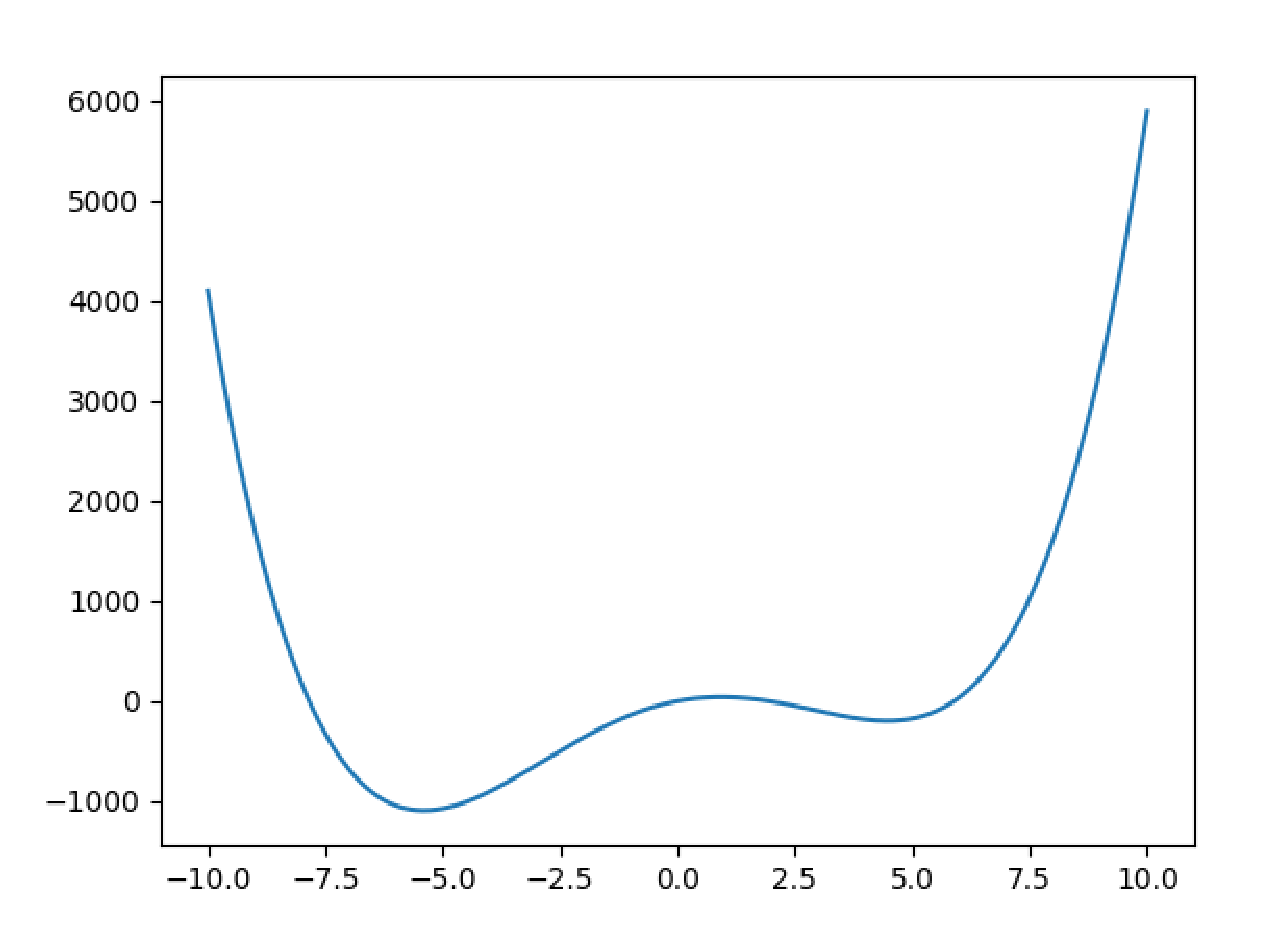
\includegraphics[scale=0.7]{annex/exemp}
				\caption{pas = 1, abscisse actuelle : 5.0}
				\label{exemple}
			\end{figure}\p

			Il faut par contre faire attention à ne pas avoir un taux d'apprentissage trop élevé no plus parce que nous avons aussi la possibilité de manquer le minimum absolu de la fonction.\p

			Il est aussi possible de faire varier le taux d'apprentissage \cite{lr}. De cette manière, avec un taux d'apprentissage variant de manière périodique, nous avons la possiblité de passer un gap trop important en augmentant le taux d'apprentissage, mais cela nous permet aussi de ne pas rater le puits recherché (lorsque le taux d'apprentissage diminue). La variation que \cite{lr} trouve la plus adaptée est celle-ci :
			\begin{figure}
				\begin{center}
					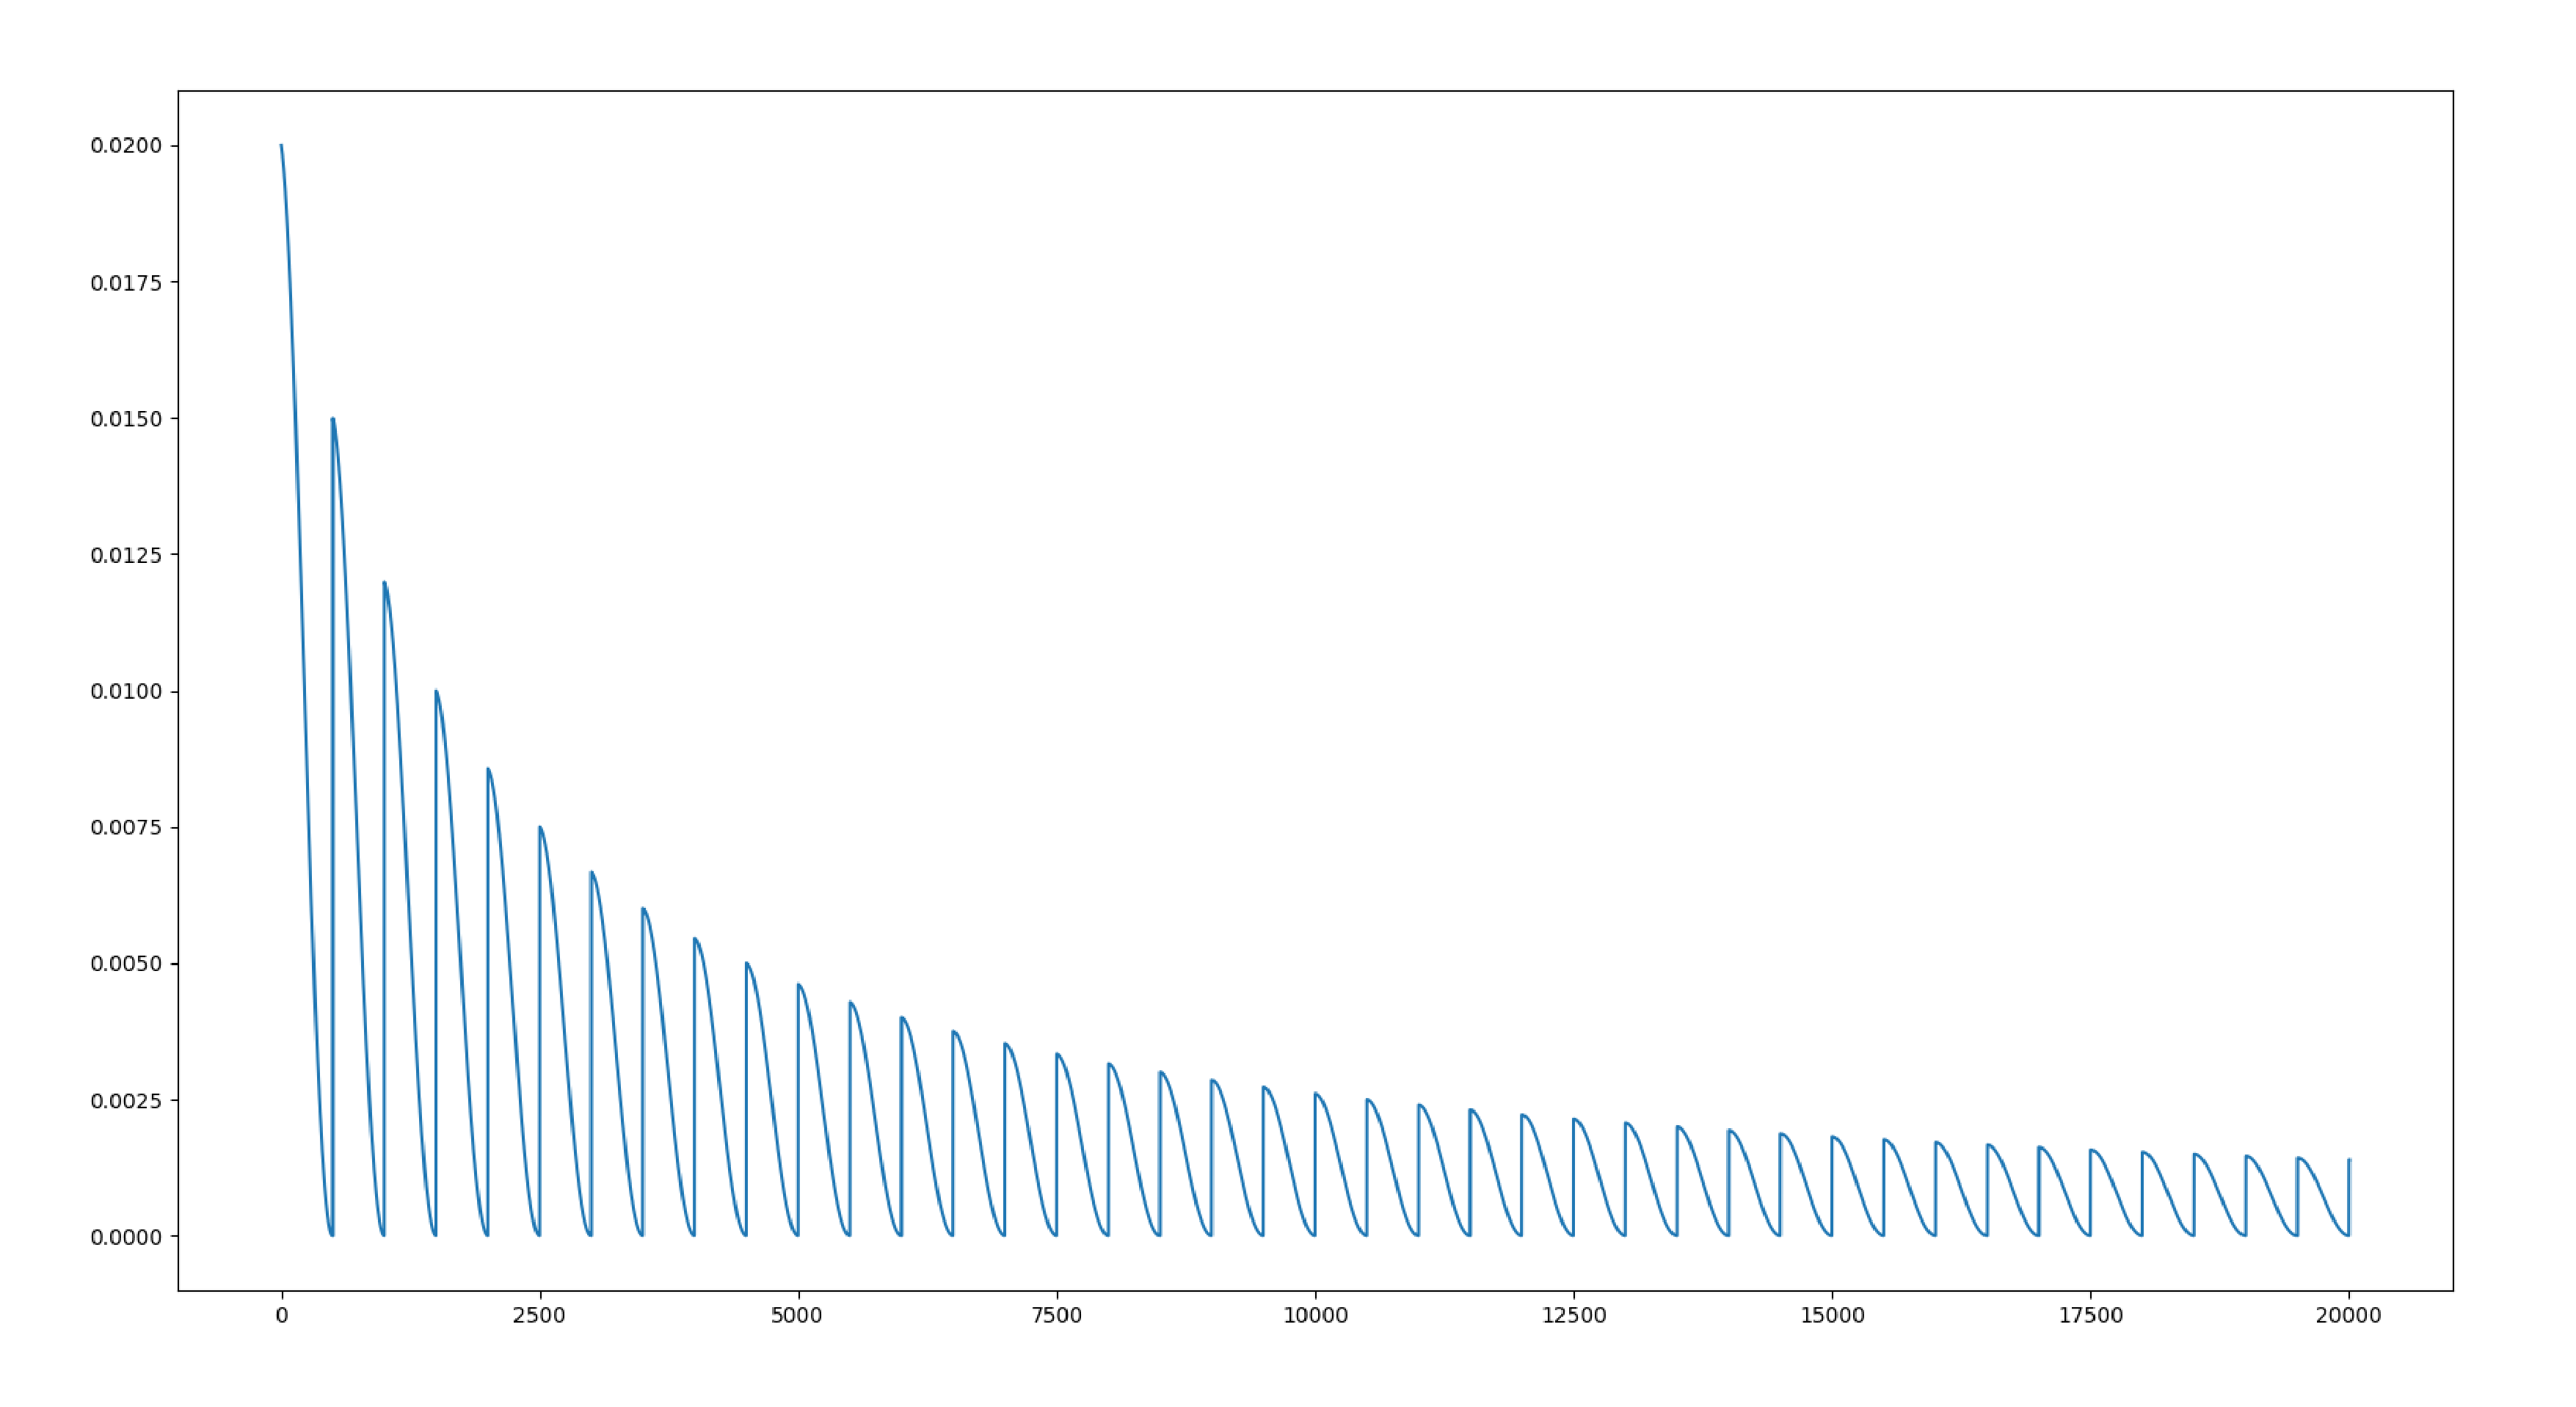
\includegraphics[scale=0.25]{annex/lr_modification}
					\caption{Modification du taux d'apprentissage à chaque itération}
					\label{ModLR}
				\end{center}
			\end{figure}

		\end{section}

  \end{chapter}

  \begin{chapter}{NiftyNet}

    NiftyNet est un projet open-source en Python qui permet de réaliser des réseaux de neurones en Deep Learning sans écrire une seule ligne de Python. Il permet à l'aide d'un fichier de configuration (fichier INI) d'entraîner des réseaux de neurones et de réaliser des prédictions après cet entraînement.\p

    Ce projet a été réalisé spécifiquement pour le domaine médical, et plus particulièrement pour le domaine de l'imagerie médicale.\p

    NiftyNet s'appuie énormément sur TensorFlow pour fonctionner.\p

  \end{chapter}

  \nocite{*}
  \bibliographystyle{plain}
  \bibliography{annex/biblio_stage}
  \addcontentsline{toc}{chapter}{Bibliographie}

\end{document}
